\documentclass{article}
\usepackage[margin=0.75in]{geometry}
\usepackage{amsmath}
\usepackage{amssymb}
\usepackage{float}
\usepackage{graphicx}

\title{Solutions to Assignment 1 : CS6510 - Applied Machine Learning}
\author{Vishwak S\\
\texttt{CS15BTECH11043}}
\date{}

\begin{document}
\maketitle

\section*{Question 1}
\subsection*{Part 1}
\begin{flushleft}
Since \(X\) and \(Y\) are independent, \(P(X)\times P(Y) = P(X \cap Y)\). \(P(\bar{X}) = 1 - P(X)\). Due to this:
\begin{gather*}
P(\bar{X} \cap Y) = P(Y) - P(X \cap Y) \quad \text{ (from Set Theory)} \\
\implies P(\bar{X} \cap Y) = P(Y) - P(Y)\times P(X) = P(Y)(1 - P(X)) = P(Y) \times P(\bar{X}) 
\end{gather*}

Hence \(\bar{X}\) and \(Y\) are independent.
\end{flushleft}

\subsection*{Part 2}
\begin{flushleft}
Listing down the information from the question:
\begin{center}
\begin{tabular}{c c c c}
\(P(C1 = H) \) & \(= 0.5\) & \(P(C1 = T) \) & \( = 0.5\) \\
\(P(C2 = H | C1 = H) \) & \(= 0.7\) & \(P(C2 = H | C1 = T) \) & \( = 0.5\) 
\end{tabular}
\end{center}

From Bayes' Theorem: \(P(A | B) = \displaystyle \frac{P(B | A) P(A)}{P(B)}\). We need to find: \(P(C1 = T \cap C2 = H | S = 1)\).
\begin{gather*}
\displaystyle P(C1 = T \cap C2 = H | S = 1) = \frac{P(C1 = T \cap C2 = H) P(S = 1 | C1 = T \cap C2 = H)}{P(S = 1)} \quad \text{ (from Bayes' Theorem)} \\
\implies \displaystyle P(C1 = T \cap C2 = H | S = 1) = \frac{P(C2 = H | C1 = T) P(C1 = T) \times 1}{P(C2 = H \cap C1 = T) + P(C2 = T \cap C1 = H)} \quad \text{ (from Cond. Probability)} \\
\implies \displaystyle P(C1 = T \cap C2 = H | S = 1) = \frac{0.5 \times 0.5}{P(C2 = H | C1 = T) P(C1 = T) + P(C2 = T | C1 = H) P(C1 = H)} \\
\implies \displaystyle P(C1 = T \cap C2 = H | S = 1) = \frac{0.25}{0.5 \times 0.5 + 0.3 \times 0.5} = \frac{5}{8} = \boxed{0.625}
\end{gather*}
\end{flushleft}

\section*{Question 2}
\subsection*{Part a}
\begin{flushleft}
A set \(S\) is a vector space if the following conditions hold:
\begin{itemize}
\item if \(u, v \in S\), then \(u + v \in S\).
\item if \(u \in S\), then \(\alpha u \in S \quad \forall \alpha\).
\end{itemize}

\(\nexists u, v \in S = \emptyset\), hence the first condition holds [\texttt{False} \(\implies\) \texttt{True} is \texttt{True}]. Similarly, \(\nexists u \in S = \emptyset\), hence the second condition holds for the same reason above. Hence the empty set is a vector space.
\end{flushleft}

\subsection*{Part b and c}
\begin{flushleft}
Let \(M^{-1}\) be of the form: \(I + \alpha(\mathbf{u} \mathbf{v}^{T})\). We know that: \(M M^{-1} = I\). Applying this we get:
\begin{gather*}
M  M^{-1} = I \\
(I + \mathbf{u}\mathbf{v}^T) (I + \alpha(\mathbf{u}\mathbf{v}^{T})) = I \\
\implies I + \mathbf{u}\mathbf{v}^{T}(1 + \alpha) + \alpha\mathbf{u}(\mathbf{v}^{T} \mathbf{u})\mathbf{v}^{T} = I \\
\implies \mathbf{u}\mathbf{v}^{T}\left((1 + \alpha) + \alpha(\mathbf{v}^{T}\mathbf{u})\right) = \mathbf{0} \\
\implies \alpha = \displaystyle \frac{-1}{1 + \mathbf{v}^{T} \mathbf{u}} 
\end{gather*}

Since there is an \(\alpha\), we can tell that our assumption is true, and hence the inverse of the matrix \(M\) is of the form \(I + \alpha(\mathbf{u}\mathbf{v}^{T})\). 
\end{flushleft}

\subsection*{Part d and e}
\begin{flushleft}
If \(M\) is singular: then \(\text{det}M = 0\). We know that the eigenvalues of \(M = I + \mathbf{u}\mathbf{v}^{T}\) are of the form: \(1 + \lambda_{i}\), where \(\lambda_{i}\)s are the eigenvalues of \(\mathbf{u}\mathbf{v}^{T}\). We also know that the determinant of the matrix is the product of its eigenvalues.
\begin{gather*}
\text{det}M = 0 \implies \displaystyle \prod_{i=1}^{n} (1 + \lambda_{i}) = 0 \\
\implies \exists \lambda_{k} \text{ such that }(1 + \lambda_{k}) = 0
\end{gather*}

This means that at least one of the eigenvalues of \(\mathbf{u}\mathbf{v}^{T}\) is exactly \(-1\). From the expression for \(\alpha\), we know that this definitely happens when \(\mathbf{v}^{T} \mathbf{u} = -1\), in which case, \(\alpha\) is undefined. 
\(\newline\)

The Null space of \(M\) is defined as: \(M \mathbf{x} = \mathbf{0}\). This means that:
\begin{gather*}
(I + \mathbf{u}\mathbf{v}^{T}) \mathbf{x} = \mathbf{0} \\
\mathbf{x} + \mathbf{u}\mathbf{v}^{T} \mathbf{x} = \mathbf{0} 
\end{gather*}

Recall that if \(M\) is singular, then \(-1\) is an eigenvalue of \(\mathbf{u} \mathbf{v}^{T}\) and hence: \(\mathbf{u}\mathbf{v}^{T}\mathbf{x} = -\mathbf{x}\). 

Resuming from where we left off: consider \(\mathbf{x} = \mathbf{u}\). \(\mathbf{u} - \mathbf{u} = 0 \text{ (since }\mathbf{v}^{T}\mathbf{u} = -1 \text{)} \).
\end{flushleft}

\section*{Question 3}
\subsection*{Part a}
\begin{flushleft}
\begin{equation*}
A = \begin{bmatrix} 
-2 & 2 \\
-6 & 5
\end{bmatrix}
\end{equation*}

The eigenvalues of \(A\) are given by the roots to the equation \(\text{det}(A - \lambda I) = 0\). We get: \(\lambda^2 - 3\lambda + 2 = 0 \implies \lambda = 1, 2\). The eigenvectors are solutions to the equation:
\begin{equation*}
A \mathbf{x} = \lambda_{i} \mathbf{x} 
\end{equation*}

For \(\lambda = 1\):
\begin{gather*}
A \mathbf{x} = \mathbf{x} \implies \begin{bmatrix} -2 & 2 \\ -6 & 5 \end{bmatrix} \begin{bmatrix} a \\ b \end{bmatrix} = \begin{bmatrix} a \\ b \end{bmatrix} \\
\mathbf{x} = a \begin{bmatrix} 1 \\ \frac{3}{2} \end{bmatrix} \quad \forall a
\end{gather*}

For \(\lambda = 2\):
\begin{gather*}
A \mathbf{x} = 2\mathbf{x} \implies \begin{bmatrix} -2 & 2 \\ -6 & 5 \end{bmatrix} \begin{bmatrix} a \\ b \end{bmatrix} = \begin{bmatrix} 2a \\ 2b \end{bmatrix} \\
\mathbf{x} = a \begin{bmatrix} 1 \\ 2 \end{bmatrix} \quad \forall a
\end{gather*}
\end{flushleft}

\subsection*{Part b}
\begin{flushleft}
Let \(U = \begin{bmatrix} u_{1} & u_{2} \\ u_{3} & u_{4} \end{bmatrix}\).
Solving the system:
\begin{gather*}
AU = U\Lambda \\
\implies u_{3} = 3\frac{u_{1}}{2} \text{ and } u_{4} = 2u_{2} \\
\end{gather*}

\(U\) is the matrix of the eigenvectors of \(A\). For simplicity, consider: \(u_{1} = 2\gamma, u_{2} = \zeta \implies u_{3} = 3\gamma, u_{4} = 2\zeta\). Hence:
\begin{equation*}
U = \begin{bmatrix}
2\gamma & \zeta \\ 3\gamma & 2\zeta 
\end{bmatrix}
\end{equation*}
\end{flushleft}

\subsection*{Part c}
\begin{flushleft}
For an invertible \(2 \times 2\) matrix \(A = \begin{bmatrix} a & b \\ c & d \end{bmatrix}\), the inverse is:
\begin{equation*}
A^{-1} = \frac{1}{ad - bc} \begin{bmatrix} d & -b \\ -c & a \end{bmatrix} 
\end{equation*}

This can be found using the transpose of the co-factor matrix (adjoint). In our case:
\begin{gather*}
U^{-1} = \frac{1}{\gamma \zeta} \begin{bmatrix} \zeta & -\zeta \\ -3\gamma & 2\gamma \end{bmatrix} \\
U\Lambda U^{-1} = \begin{bmatrix} 2\gamma & 2\zeta \\ 3\gamma & 4\zeta \end{bmatrix} \begin{bmatrix} 1 & 0 \\ 0 & 2 \end{bmatrix} \begin{bmatrix} 2\zeta & -\zeta \\ -3\gamma & 2\gamma \end{bmatrix} \frac{1}{\gamma \zeta}\\
\implies U\Lambda U^{-1} = \begin{bmatrix} 2\gamma & 2\zeta \\ 3\gamma & 4 \zeta \end{bmatrix} \begin{bmatrix} 2\zeta & -\zeta \\ -3\gamma & 2\gamma \end{bmatrix} \frac{1}{\gamma \zeta} = \frac{1}{\gamma \zeta} \begin{bmatrix} -2\gamma \zeta & 2\gamma \zeta \\ -6\gamma \zeta & 5\gamma\zeta\end{bmatrix} \\
\implies U\Lambda U^{-1} = \begin{bmatrix} -2 & 2 \\ -6 & 5 \end{bmatrix} = A
\end{gather*}

Verified. 
\end{flushleft}

\section*{Question 4}
\subsection*{Part a}
\begin{flushleft}
When you are calculating the training loss, the entire training set is taken into account. Hence while predicting the class for a particular \(\mathbf{x}_{i}\) in the training set, the closest neighbour to \(\mathbf{x}_{i}\) is itself. Hence if \(k=1\), then the training loss is \(0\) (considering a zero-one loss).
\(\newline\)

In general it can be said that the loss is expected to have an increasing trend as \(k\) increases. But when \(k = n\), then the majority class is given. In our case, there is no majority class, hence the labelling might depend on the ordering of the data. \(\frac{n}{2}\) points will be given the opposite class, hence the training loss will be \(\frac{n}{2}\) (again considering a zero-one loss).
\end{flushleft}

\subsection*{Part b}
\begin{flushleft}
We can expect the loss to vary in a parabolic sense. This is shown in the sketch below:
\begin{figure}[H]
\centering
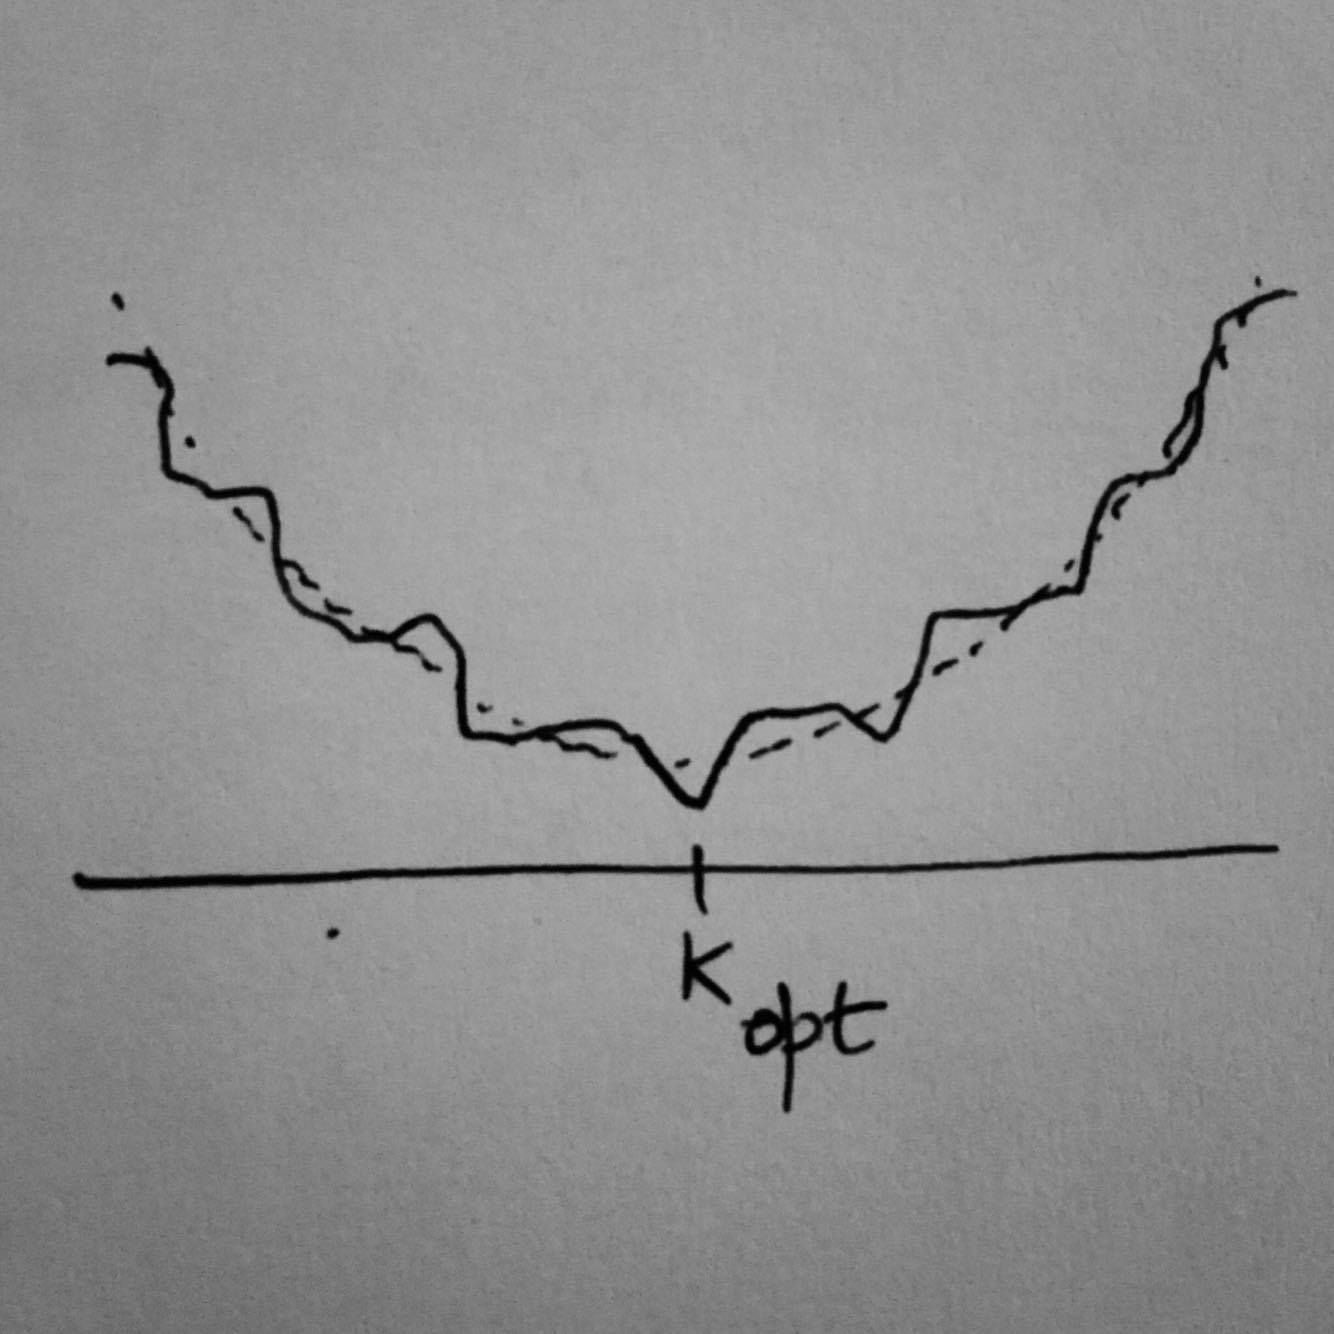
\includegraphics[width=0.3\linewidth]{4b.jpg}
\caption{The dotted lines represent a smoothened behaviour of the thick line depicting a possible variation in the testing loss (assuming zero-one loss)}
\end{figure}

Although this is a general opinion, the exact variation of the test loss will depend on the similarities of distribution of the training and testing set. But if \(k\) is too-small, then we become more sensitive to the noise in the data. On the contrary, if \(k\) is too large, then we begin to get attributes for other classes. Hence the parabolic nature of the plot.
\end{flushleft}

\subsection*{Part c}
\begin{flushleft}
\begin{itemize}
\item If the dimensionality is too high, there are higher computation costs to evaluate the "distance" between two points and also storing them. Coupled with the fact that you need to run through the entire training set to make predictions, this is one disadvantage of k-NN.
\item If the dimensionality is high, it can be shown mathematically that the concentration of points are higher close to the surface than in the volume. This is known as the curse of dimensionality. Due to this, the neighbours of a given point are actually not close anymore, meaning that the neighbours of that point are actually far which may influence the class of the given point.
\end{itemize}
\end{flushleft}

\subsection*{Part d}
\begin{flushleft}
It is possible to generate a tree to match the \underline{training} predictions of a 1-NN classifier. All we need is fully-constructed univariate decision tree. However it is generally impossible to match the decision boundary of 1-NN classifier. The 1-NN classifier has decision boundaries depicted by a Voronoi diagram (which are in some sense polyhedral), whereas the decision boundaries for a decision tree with the decisions as inequalities would be boxes with sides parallel to the axes. Due to the existence of difference in the decision boundary, the generalization performance may be different.
\end{flushleft}

\section*{Question 5}
\subsection*{Part a}
\begin{flushleft}
Since we want multi-way splits, we are taking \texttt{Airbag} into account. We find the best among \texttt{Price}, \texttt{Maintenance} and \texttt{Capacity}. For this we first calculate the impurity after splitting and then we calculate the information gain.
\(\newline\)

For \texttt{Price}, the split gives: 
\begin{equation*}
\boxed{\text{Price (6: Y, 5: N)}} \rightarrow \boxed{\text{Low(L) (2: yes, 2: no)}}, \boxed{\text{Medium(M) (2: Y, 2: N)}} \text{ and } \boxed{\text{High(H) (2: Y, 1: N)}}
\end{equation*}
Impurity after split:
\begin{gather*}
\displaystyle \text{Imp}_{\text{Price}} = -\left(\frac{n_{\text{L}}}{n}\left(\sum_{i = \{Y, N\}} p_{i | \text{L}}\log_{2}(p_{i | \text{L}})\right) + \frac{n_{\text{M}}}{n}\left(\sum_{i = \{Y, N\}} p_{i | \text{M}}\log_{2}(p_{i | \text{M}})\right) + \frac{n_{\text{H}}}{n}\left(\sum_{i = \{Y, N\}} p_{i | \text{H}}\log_{2}(p_{i | \text{H}})\right) \right) \\
\implies \displaystyle \text{Imp}_{\text{Price}} = -\left(\frac{4}{11}\left(\frac{1}{2}\log_{2}\frac{1}{2} + \frac{1}{2}\log_{2}\frac{1}{2}\right) + \frac{4}{11}\left(\frac{1}{2}\log_{2}\frac{1}{2} + \frac{1}{2}\log_{2}\frac{1}{2}\right) + \frac{3}{11}\left(\frac{2}{3}\log_{2}\frac{2}{3} + \frac{1}{3}\log_{2}\frac{1}{3}\right)\right) \\
\implies \text{Imp}_{\text{Price}} \approx \mathbf{0.9778}
\end{gather*}

For \texttt{Maintenance}, the split gives:
\begin{equation*}
\boxed{\text{Maintain (6: Y, 5: N)}} \rightarrow \boxed{\text{Low(L) (2: yes, 0: no)}}, \boxed{\text{Medium(M) (2: Y, 2: N)}} \text{ and } \boxed{\text{High(H) (2: Y, 3: N)}}
\end{equation*}
Impurity after split:
\begin{gather*}
\displaystyle \text{Imp}_{\text{Maintain}} = -\left(\frac{n_{\text{L}}}{n}\left(\sum_{i = \{Y, N\}} p_{i | \text{L}}\log_{2}(p_{i | \text{L}})\right) + \frac{n_{\text{M}}}{n}\left(\sum_{i = \{Y, N\}} p_{i | \text{M}}\log_{2}(p_{i | \text{M}})\right) + \frac{n_{\text{H}}}{n}\left(\sum_{i = \{Y, N\}} p_{i | \text{H}}\log_{2}(p_{i | \text{H}})\right) \right) \\
\implies \displaystyle \text{Imp}_{\text{Maintain}} = -\left(\frac{2}{11}\left(1\log_{2}1 + 0\log_{2}0\right) + \frac{4}{11}\left(\frac{1}{2}\log_{2}\frac{1}{2} + \frac{1}{2}\log_{2}\frac{1}{2}\right) + \frac{5}{11}\left(\frac{2}{5}\log_{2}\frac{2}{5} + \frac{3}{5}\log_{2}\frac{3}{5}\right)\right) \\
\implies \text{Imp}_{\text{Maintain}} \approx \mathbf{0.8050}
\end{gather*}

For \texttt{Capacity}, the split gives:
\begin{equation*}
\boxed{\text{Capacity (6: Y, 5: N)}} \rightarrow \boxed{\text{2 (1: yes, 2: no)}}, \boxed{\text{4 (3: Y, 3: N)}} \text{ and } \boxed{\text{5 (2: Y, 0: N)}}
\end{equation*}
Impurity after split:
\begin{gather*}
\displaystyle \text{Imp}_{\text{Capacity}} = -\left(\frac{n_{\text{2}}}{n}\left(\sum_{i = \{Y, N\}} p_{i | \text{2}}\log_{2}(p_{i | \text{2}})\right) + \frac{n_{\text{4}}}{n}\left(\sum_{i = \{Y, N\}} p_{i | \text{4}}\log_{2}(p_{i | \text{4}})\right) + \frac{n_{\text{5}}}{n}\left(\sum_{i = \{Y, N\}} p_{i | \text{5}}\log_{2}(p_{i | \text{5}})\right) \right) \\
\implies \displaystyle \text{Imp}_{\text{Capacity}} = -\left(\frac{3}{11}\left(\frac{1}{3}\log_{2}\frac{1}{3} + \frac{2}{3}\log_{2}\frac{2}{3}\right) + \frac{6}{11}\left(\frac{1}{2}\log_{2}\frac{1}{2} + \frac{1}{2}\log_{2}\frac{1}{2}\right) + \frac{2}{11}\left(1\log_{2}1 + 0\log_{2}0\right)\right) \\
\implies \text{Imp}_{\text{Capacity}} \approx \mathbf{0.7959}
\end{gather*}

Now the impurity at the root is given by: \(\text{Imp}_{\text{root}} = \displaystyle -\frac{6}{11}\log_{2}\frac{6}{11} -\frac{5}{11}\log_{2}\frac{5}{11} \approx 0.994\).
\(\newline\)

The information gain for every split is:
\begin{center}
\begin{tabular}{|c|c|}
\hline
Split & Inf. Gain \\
\hline
\texttt{Price} & \(0.994 - 0.9778 = 0.0163\) \\
\hline
\texttt{Maintenance} & \(0.994 - 0.8050 = 0.189\) \\
\hline
\texttt{Capacity} & \(0.994 - 0.7959 = 0.1981\) \\
\hline 
\end{tabular}
\end{center}

From this, it is evident that splitting at \textbf{Capacity} gives us better information gain.
\end{flushleft}
\subsection*{Part b}
\begin{flushleft}
Since we are taking into account binary splitting, below listed are the possible choices of splits:
\begin{enumerate}
\item \texttt{Price}(6: Y, 5: N) \(\rightarrow\) \texttt{Low}(2: Y, 2: N) and \texttt{Medium | High}(4: Y, 3: N) 
\item \texttt{Price}(6: Y, 5: N) \(\rightarrow\) \texttt{Medium}(2: Y, 2: N) and \texttt{High | Low}(4: Y, 3: N)
\item \texttt{Price}(6: Y, 5: N) \(\rightarrow\) \texttt{High}(2: Y, 1: N) and \texttt{Low | Medium}(4: Y, 4: N)
\item \texttt{Maintenance}(6: Y, 5: N) \(\rightarrow\) \texttt{Low}(2: Y, 0: N) and \texttt{Medium | High}(4: Y, 5: N)
\item \texttt{Maintenance}(6: Y, 5: N) \(\rightarrow\) \texttt{Medium}(2: Y, 2: N) and \texttt{High | Low}(4: Y, 3: N)
\item \texttt{Maintenance}(6: Y, 5: N) \(\rightarrow\) \texttt{High}(2: Y, 3: N) and \texttt{Low | Medium}(4: Y, 2: N)
\item \texttt{Capacity}(6: Y, 5: N) \(\rightarrow\) \texttt{2}(1: Y, 2: N) and \texttt{4 | 5}(5: Y, 3: N)
\item \texttt{Capacity}(6: Y, 5: N) \(\rightarrow\) \texttt{4}(3: Y, 3: N) and \texttt{5 | 2}(3: Y, 2: N)
\item \texttt{Capacity}(6: Y, 5: N) \(\rightarrow\) \texttt{5}(2: Y, 0: N) and \texttt{2 | 4}(4: Y, 5: N)
\item \texttt{Airbag}(6: Y, 5: N) \(\rightarrow\) \texttt{Yes}(3: Y, 3: N) and \texttt{No}(3: Y, 2: N)
\end{enumerate}

Impurities for 1, 2 and 5 will be same due to same distribution of the labels. Similarly impurities for 4 and 9 will be same, and it is the same case for 8 and 10.
Calculating the impurity for 1 (and 2, 5):
\begin{gather*}
\text{Imp}_{1} = \left(\frac{n_{\text{L}}}{n} \left(1 - \sum_{i = \{Y, N\}} p_{i | \text{L}}^{2}\right) + \frac{n_{\text{M or H}}}{n} \left(1 - \sum_{i = \{Y, N\}} p_{i | \text{M or H}}^{2}\right)\right) \\
\text{Imp}_{1} = \left(\frac{4}{11} \left(1 - \frac{1}{4} - \frac{1}{4}\right) + \frac{7}{11} \left(1 - \frac{16}{49} - \frac{9}{49}\right)\right) \\
\text{Imp}_{1} \approx \mathbf{0 4935}
\end{gather*}

Calculating the impurity for 3:
\begin{gather*}
\text{Imp}_{3} = \left(\frac{n_{\text{H}}}{n} \left(1 - \sum_{i = \{Y, N\}} p_{i | \text{H}}^{2}\right) + \frac{n_{\text{L or M}}}{n} \left(1 - \sum_{i = \{Y, N\}} p_{i | \text{L or M}}^{2}\right)\right) \\
\text{Imp}_{3} = \left(\frac{3}{11} \left(1 - \frac{4}{9} - \frac{1}{9}\right) + \frac{8}{11} \left(1 - \frac{1}{4} - \frac{1}{4}\right)\right) \\
\text{Imp}_{3} \approx \mathbf{0.4849} 
\end{gather*}

Calculating the impurity for 4 (and 9):
\begin{gather*}
\text{Imp}_{4} = \left(\frac{n_{\text{L}}}{n} \left(1 - \sum_{i = \{Y, N\}} p_{i | \text{L}}^{2}\right) + \frac{n_{\text{M or H}}}{n} \left(1 - \sum_{i = \{Y, N\}} p_{i | \text{M or H}}^{2}\right)\right) \\
\text{Imp}_{4} = \left(\frac{2}{11} \left(1 - 1 - 0\right) + \frac{9}{11} \left(1 - \frac{16}{81} - \frac{25}{81}\right)\right) \\
\text{Imp}_{4} \approx \mathbf{0.4040} 
\end{gather*}

Calculating the impurity for 6:
\begin{gather*}
\text{Imp}_{6} = \left(\frac{n_{\text{H}}}{n} \left(1 - \sum_{i = \{Y, N\}} p_{i | \text{H}}^{2}\right) + \frac{n_{\text{L or M}}}{n} \left(1 - \sum_{i = \{Y, N\}} p_{i | \text{Lor M}}^{2}\right)\right) \\
\text{Imp}_{6} = \left(\frac{5}{11} \left(1 - \frac{4}{25} - \frac{9}{25}\right) + \frac{6}{11} \left(1 - \frac{4}{9} - \frac{1}{9}\right)\right) \\
\text{Imp}_{6} \approx \mathbf{0.4606} 
\end{gather*}

Calculating the impurity for 7:
\begin{gather*}
\text{Imp}_{7} = \left(\frac{n_{\text{2}}}{n} \left(1 - \sum_{i = \{Y, N\}} p_{i | \text{2}}^{2}\right) + \frac{n_{\text{4 or 5}}}{n} \left(1 - \sum_{i = \{Y, N\}} p_{i | \text{4 or 5}}^{2}\right)\right) \\
\text{Imp}_{7} = \left(\frac{3}{11} \left(1 - \frac{1}{9} - \frac{4}{9}\right) + \frac{8}{11} \left(1 - \frac{25}{64} - \frac{9}{64}\right)\right) \\
\text{Imp}_{7} \approx \mathbf{0.4621} 
\end{gather*}

Calculating the impurity for 8 (and 10):
\begin{gather*}
\text{Imp}_{8} = \left(\frac{n_{\text{4}}}{n} \left(1 - \sum_{i = \{Y, N\}} p_{i | \text{4}}^{2}\right) + \frac{n_{\text{5 or 2}}}{n} \left(1 - \sum_{i = \{Y, N\}} p_{i | \text{5 or 2}}^{2}\right)\right) \\
\text{Imp}_{8} = \left(\frac{6}{11} \left(1 - \frac{1}{4} - \frac{1}{4}\right) + \frac{5}{11} \left(1 - \frac{9}{25} - \frac{4}{25}\right)\right) \\
\text{Imp}_{8} \approx \mathbf{0.4909} 
\end{gather*}

Impurity at the root for any split:  \(\text{Imp}_{\text{root}} = \displaystyle 1 - \frac{36}{121} - \frac{25}{121} = \mathbf{0.4957}\).
Information gain table below:
\begin{center}
\begin{tabular}{|c|c|c|c|}
\hline
Split number & Inf. gain & Split number & Inf. gain \\
\hline
1 & 0.0024 & 6 & 0.0353 \\
\hline
2 & 0.0024 & 7 & 0.0338 \\
\hline
3 & 0.0110 & 8 & 0.0050 \\
\hline
4 & 0.0918 & 9 & 0.0918 \\
\hline
5 & 0.0024 & 10 & 0.0050 \\
\hline
\end{tabular}
\end{center}

Highest information gain occurs for splits \textbf{4} and \textbf{9}. 
\end{flushleft}
\end{document}
